%Welle
Der Ultraschall-Scan arbeitet mit der Ausbreitung von Schallwellen.
Schallwellen sind Longitudinalwellen der Form
\begin{align*}
  p(x, t)= p_{\text{0}}-v_{\text{0}}Z \cos{(\omega t -k x)}.
\end{align*}
Dabei ist die Größe $Z$ ist die akustische Impedanz $Z=c \cdot \rho$, also das Produkt aus Schallgeschwindigkeit $c$ und der Dichte $\rho$ des durchschallten Mediums.
Damit ist die Ausbreitung der Schallwellen direkt abhängig von der Dichte des Mediums.
\\ Die Schallwellen werden häufig durch den Piezo-elektrischen Effekt erzeugt.
Dabei wird ein Piezokristall durch ein wechselndes elektrisches Feld in Schwingung gebracht.
Diese Wellen können als Ultraschall für die Untersuchung genutzt werden.
Wird die Resonanzfrequenz des Kristalls erreicht, entstehen durch die Resonanzüberhöhung energiereiche Schallwellen.
Andersherum kann ein ruhender Piezokristall durch eine Schallwelle in Schwingung gebracht werden, die dann als Spannung in das elektrische Feld eingehen.
Damit kann der Piezo-elektrische Effekt sowohl für den Ultraschallsender und den Ultraschallempfänger verwendet werden.
%Schallgeschwindigkeit
\\Die Schallgeschwindigkeit in Flüssigkeiten und Gasen ergibt sich mit der Kompressibilität $\kappa$ zu
\begin{align}
  c_{\text{Flüssig}}=\frac{1}{\sqrt{\kappa \rho}}.
  \label{eqn:flüssig}
\end{align}
In Festkörpern kann sich der Schall auch transversal ausbreiten, dies wird hier jedoch nicht weiter betrachtet.
Die longitudinale Schallgeschwindigkeit in Festkörpern berechnet sich mit dem Elastizitätsmodul $E$:
\begin{align}
  c_{\text{Fest}}=\sqrt{\frac{E}{\rho}}.
  \label{eqn:fest}
\end{align}
Die Schallgeschwindigkeit ist also in Materialien höherer Dichte größer, als in Materialien mit niedrigeren Dichten.
Somit ist Luft im Gegensatz zu beispielsweise Wasser ein denkbar schlechter Schallleiter.
Daher wird beim Ultraschall häufig ein Kontaktmittel, wie zum Beispiel Wasser oder Kontaktgele auf Wasserbasis verwendet.
%Intensität
\\Die Intensität des Schalls fällt exponentiell mit dem Abstand ab:
\begin{align*}
  I(x)=I_{\text{0}} \exp^{\alpha x}.
\end{align*}
Der Grund für die Abschwächung ist die Absorption des Schalls.
$\alpha$ ist entsprechend der Absorptionskoeffizient.
%Reflexion
\\An den Grenzflächen zwischen zwei Medien werden die Schallwellen teilweise reflektiert und teilweise transmittiert.
Um dieses Phänomen ausdrücken zu können gibt es den Transmissionskoeffizienten $T$ und den Reflexionskoeffizienten $R$.
Die beiden Größen hängen über die Beziehung
\begin{align*}
  1=T+R
\end{align*}
zusammen.
Der Reflexionskoeffizient berechnet sich über die akustische Impedanz:
\begin{align*}
  R= \left( \frac{Z_{\text{1}}-Z_{\text{2}}}{Z_{\text{1}}+Z_{\text{2}}} \right)^2.
\end{align*}
Bei einer reflektierten Welle kann über die Laufzeit die Entfernung der Grenzfläche zum Schallkopf bestimmt werden, wenn die Schallgeschwindigkeit in dem Medium bekannt ist:
\begin{align*}
  s=\frac{c t}{2}.
\end{align*}
%Scan-Arten
\\Nun können die Ultraschall-Scans entweder über den reflektierten Teil oder den transmittierten Teil der Welle gemacht werden.
Das Durchschallungsverfahren (Abb. \ref{fig:durchschall}) arbeitet mit dem transmittierten Teil.
Dabei werden Schallsender und Schallempfänger auf den gegenüberliegenden Seiten des zu untersuchenden Objekts angebracht.
Dabei wird die Intensität und die Laufzeit der durchdringenden Welle gemessen.
Befindet sich eine Störung im Material lässt sich die Lokalisation dieser durch das Durschschallungsverfahren nur in der Ebene herausfinden, in der der Schallsender und Schallempfänger liegen.
\\Bei dem Impuls-Echo-Verfahren (Abb. \ref{fig:impecho}) befinden sich Sender und Empfänger im gleichen Gerät.
Der Empfänger misst die Intensität und die Laufzeit der reflektierten Welle, also das Echo der gesendeten Welle.
Eine eventuelle Störung lässt sich in zwei Ebenen beschreiben, so zeigt die Laufzeitmessung genau an, wie tief die Störung im Material ist.

\begin{figure}[h!]
 \centering
 \begin{subfigure}{0.49\textwidth}
  \centering
  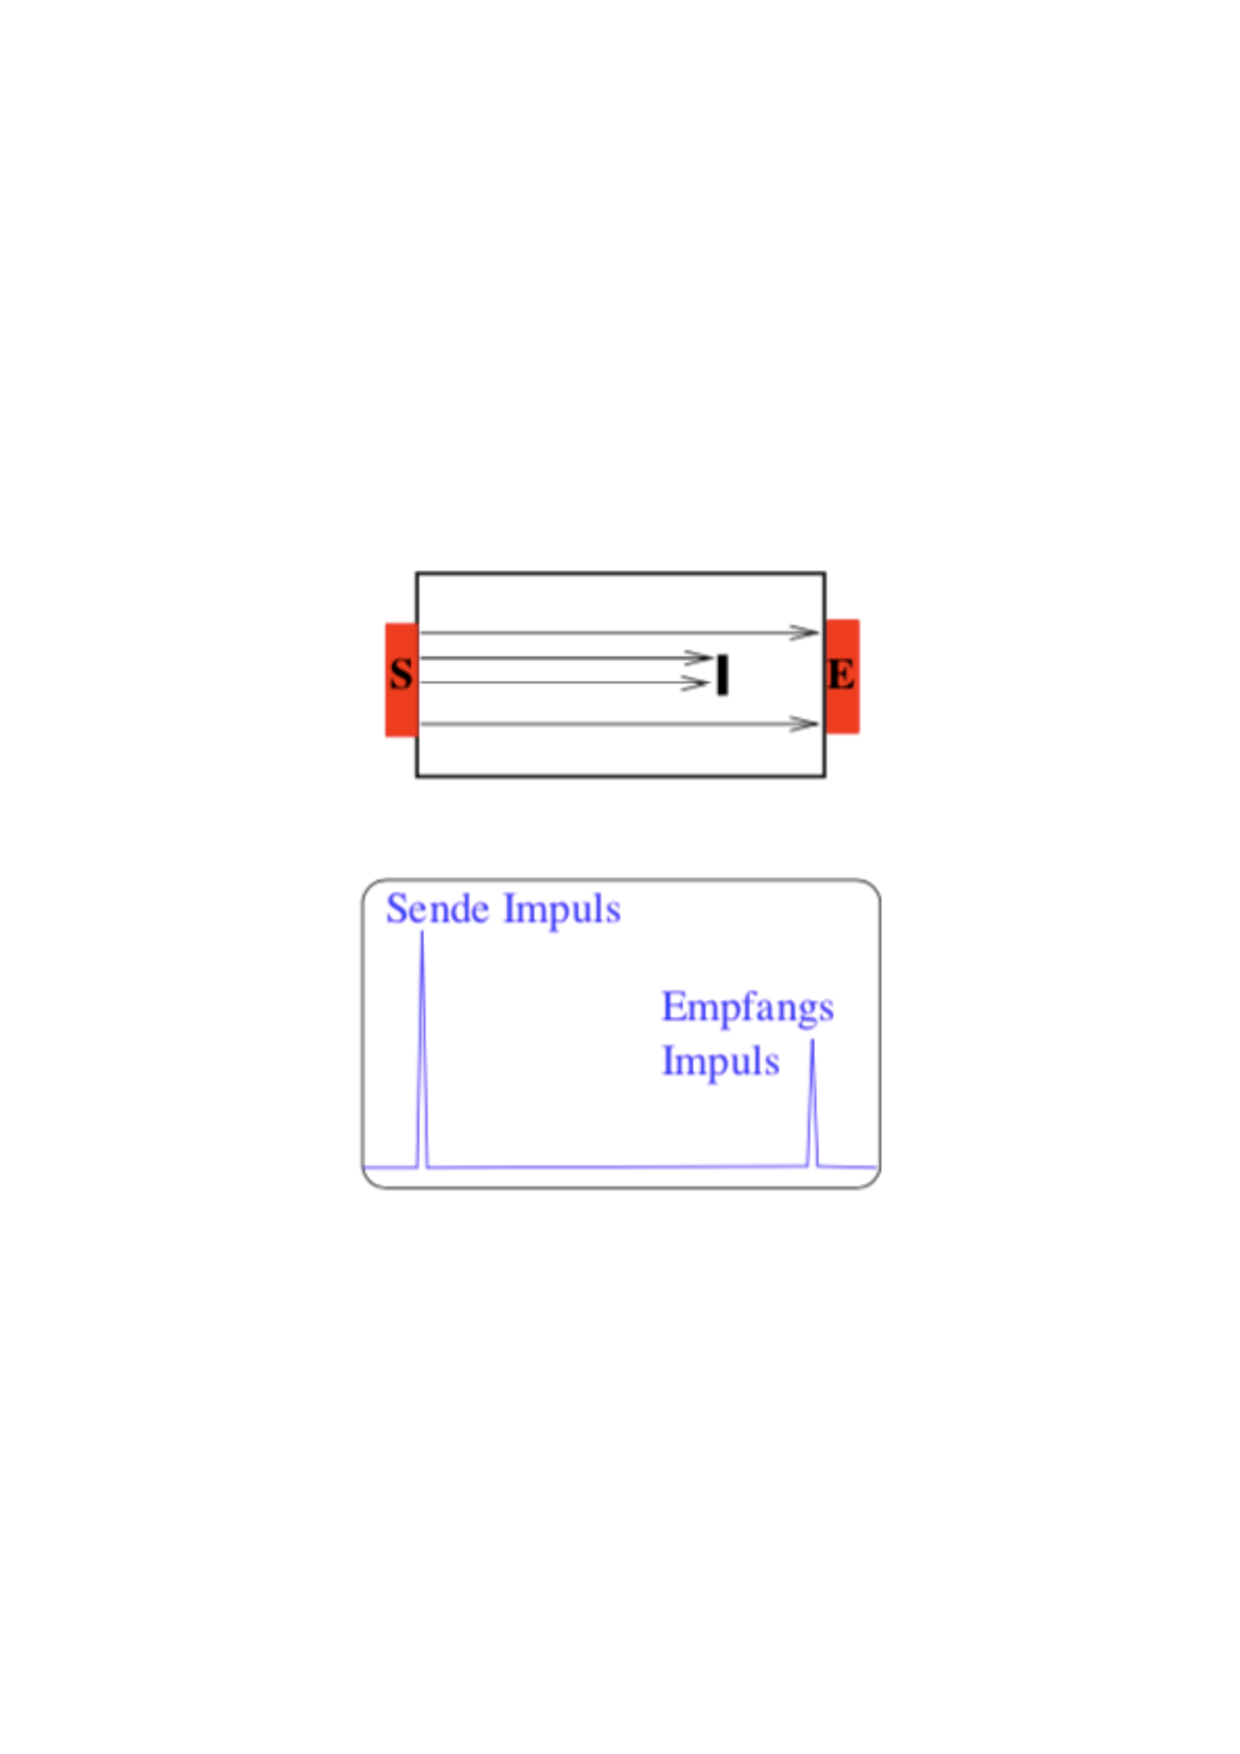
\includegraphics[width=0.9\textwidth]{durchschall.pdf}
  \caption{Durchschallungsverfahren \cite{1}}
  \label{fig:durchschall}
 \end{subfigure}
 \begin{subfigure}{0.49\textwidth}
  \centering
  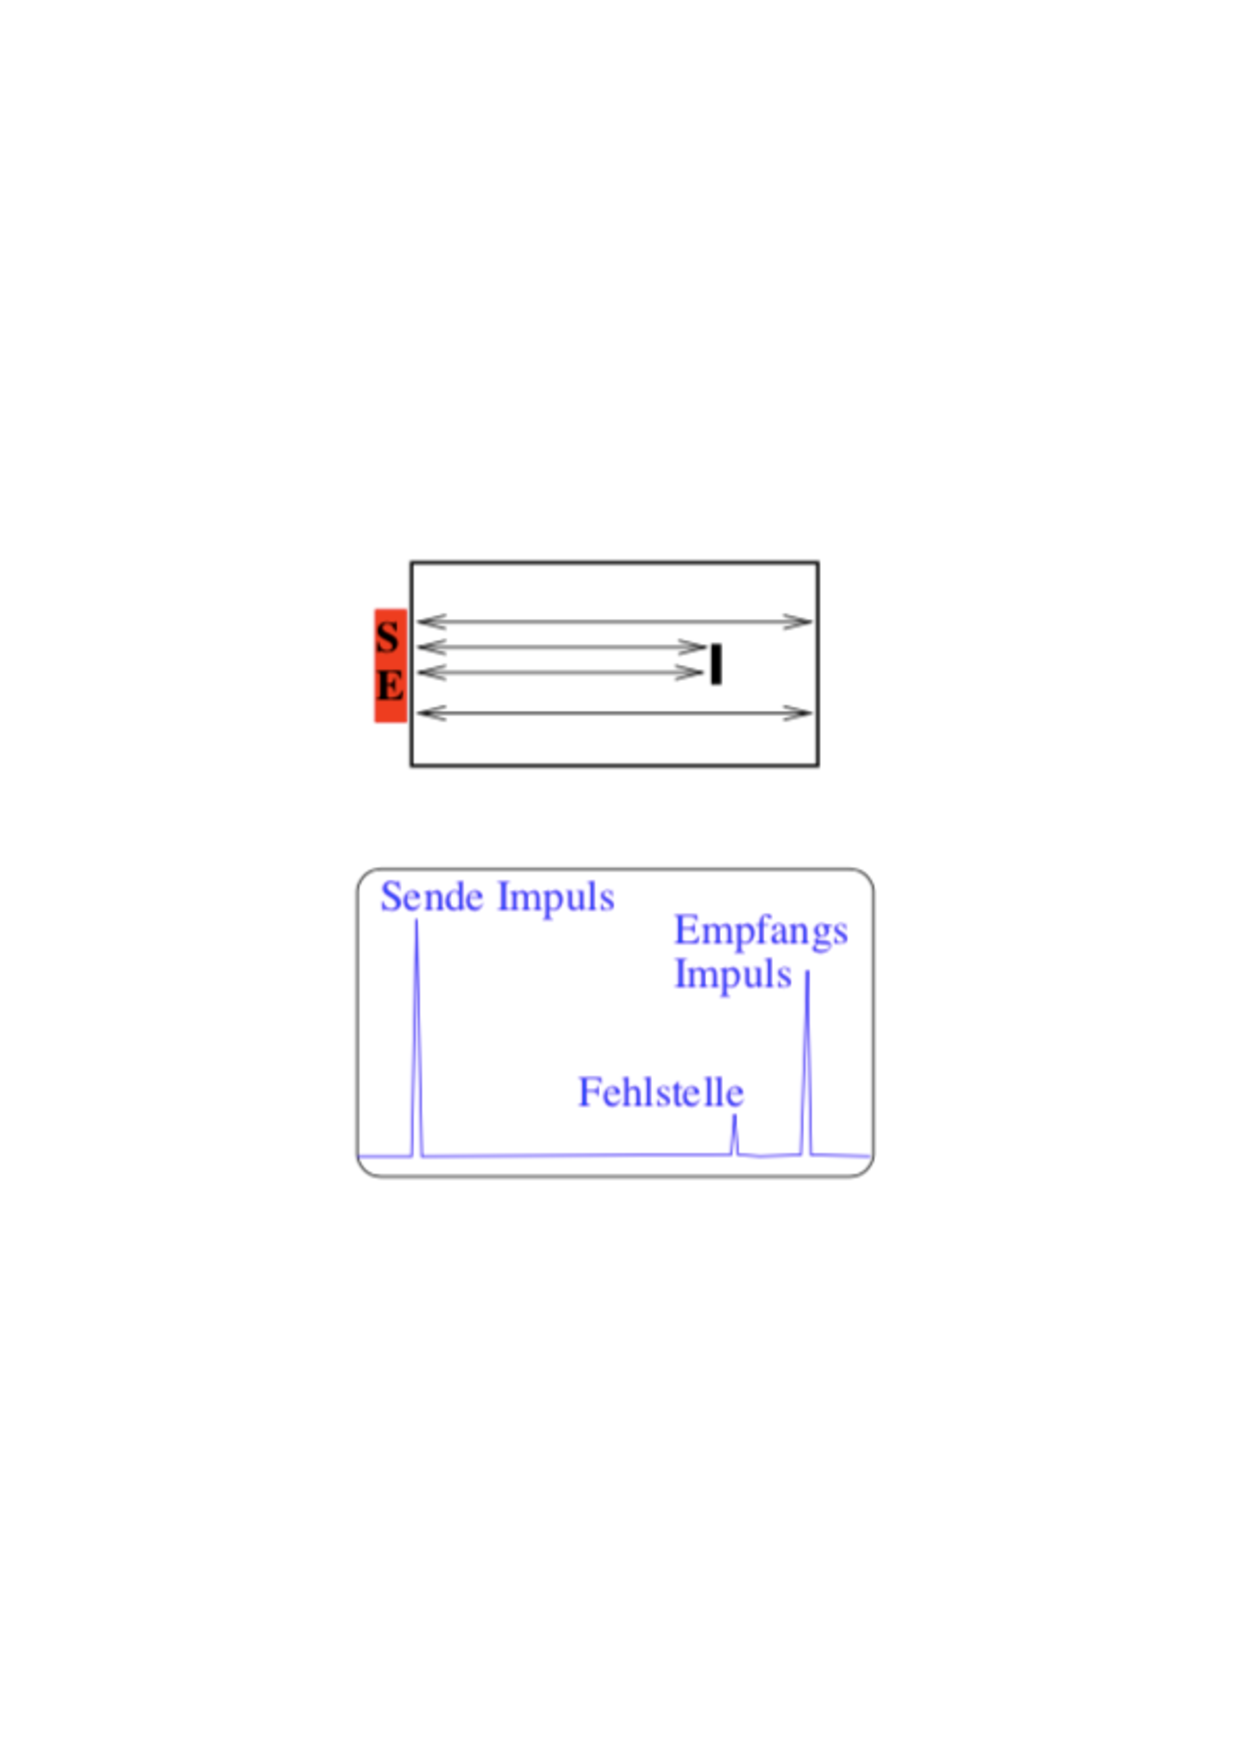
\includegraphics[width=0.9\textwidth]{impecho.pdf}
  \caption{Impuls-Echo-Verfahren \cite{1}}
  \label{fig:impecho}
 \end{subfigure}
 \caption{Verschiedene Ultraschall-Verfahren}
 \label{fig:verfahren}
\end{figure}
Die Laufzeitmessung im Impuls-Echo-Verfahren kann in drei verschiedenen Scan-Arten dargestellt werden.
\\Bei dem A-Scan werden die Laufzeiten und die Amplitude gemessen und gegeneinander aufgetragen.
Dabei entsteht ein eindimensionaler Eindruck des geschallten Körpers.
Die verschiedenen Grenzflächen sind im Diagramm als Peaks dargestellt.
\\Der B-Scan verrechnet die Informationen über die Dichte in Helligkeitsabstufungen.
Der Schallkopf wird langsam über den zu schallenden Körper bewegt.
Nun wird ein zweidimensionales Bild des Körpers erstellt.
\\Außerdem gibt es den TM-Scan.
Hier werden die Impulse sehr schnell ausgegeben, so dass auch Bewegungen im Körper zu beobachten sind.

\FloatBarrier
